\documentclass{ctexart}
\usepackage[a4paper,total={6in,8in}]{geometry}
\usepackage{fancyhdr}
\usepackage[table,xcdraw]{xcolor}
\usepackage{diagbox}
\usepackage[utf8]{inputenc}
\usepackage{ctex}
\usepackage{color}
\usepackage{subfigure}
\usepackage{cite}
\usepackage{graphicx}
\usepackage{fontspec}
\setmainfont{Times New Roman}
\newfontfamily\timesfont{Times New Roman}
\usepackage{CJK}
\usepackage{indentfirst}
\usepackage{amsmath}
\usepackage{mathrsfs}
\usepackage{multirow}
\usepackage{svg}
\usepackage{amsfonts}
\usepackage{geometry}
\usepackage{hyperref}
\usepackage{mathabx}
\usepackage{cases}
\usepackage{minipage-marginpar}
\usepackage{xcolor}
% 导入包
\usepackage{hyperref}
% 格式设置
\hypersetup{hidelinks,
	colorlinks=true,
	allcolors=blue,
	pdfstartview=Fit,
	breaklinks=true}

\begin{document}

\begin{titlepage}
    \title{{\fontsize{28}{32}\selectfont\kaishu 机器人学 \\ \fontsize{20}{24}\selectfont\kaishu{作业5:运动学轨迹规划}}}
    \date{} % delete date as you want
    \maketitle
    \vspace{-7em}
    \begin{center}
      \fontsize{18}{22}\selectfont
      \textbf{\timesfont Robotics (2023-2024-2) \\
      Homework 5: Kinematic Trajectory Planning}
    \end{center}
    
    \begin{figure}[h]
        \centering
        
\includegraphics[width=0.45\textwidth]{Image/校标-校徽.png}
    \end{figure}
    \begin{center}
      \hspace{6em}
      \renewcommand{\arraystretch}{2}
      \begin{tabular}{rl}
      \fontsize{16}{50}\selectfont\heiti 姓名:& \fontsize{16}{24}\selectfont\heiti 赵四维 \\
      \fontsize{16}{24}\selectfont\heiti 学号:& \fontsize{16}{24}\selectfont 521021910696 \\
      \fontsize{16}{24}\selectfont\heiti 班级:& \fontsize{16}{24}\selectfont ME3403-01 \\
      \fontsize{16}{24}\selectfont\timesfont E-mail:& \fontsize{16}{24}\selectfont racheus.11@sjtu.edu.cn \\
      \end{tabular}
    \end{center}
    \begin{center}
      \fontsize{16}{24}\selectfont\timesfont \today
    \end{center}
\end{titlepage}

\pagenumbering{arabic}

\newpage
% \tableofcontents


\newpage
\pagestyle{fancy}
\fancyhf{}
\fancyhead[L]{ME3403-01}
\fancyhead[C]{机器人学Homework4}
\fancyhead[R]{赵四维 521021910696}
\fancyfoot[C]{\thepage}
\section{微分运动基础}
已知坐标系{C}对基坐标系的变换为

\begin{equation}
	\begin{bmatrix}
		0 & 1 & 0 & 4\\
		0 & 0 & 1 & 3\\
		1 & 0 & 0 & 0\\
		0 & 0 & 0 & 1
	\end{bmatrix}
\end{equation}

而且对于基坐标系的微分平移分量分别为沿$x$轴移动$0.5$,沿 $y $轴移动为$0$,沿$z$ 轴移动$1$;微分旋转分量分别为 $0.1,0.2 $和 $0$。

\subsection{求相应的微分变换}
\textbf{[Solution]:}

根据题意,微分平移和旋转矢量表示为:
\begin{equation}
	\begin{aligned}
		&\mathbf{d} = 0.5\mathbf{i} + 0\mathbf{j} + 1\mathbf{k} \\
		&\mathbf{\delta} = 0.1\mathbf{i} + 0.2\mathbf{j} + 0\mathbf{k}
	\end{aligned}
\end{equation}

因此对应的$\Delta$矩阵为:
\begin{equation}
	\begin{aligned}
		\Delta = \begin{bmatrix}
			0 & -\delta_z & \delta_y & d_x \\
			\delta_z & 0 & -\delta_x & d_y \\
			-\delta_y & \delta_x & 0 & d_z \\
			0 & 0 & 0 & 0
		\end{bmatrix} = \begin{bmatrix}
			0 & 0 & 0.2 & 0.5 \\
			0 & 0 & -0.1 & 0 \\
			-0.2 & 0.1 & 0 & 1 \\
			0 & 0 & 0 & 0
		\end{bmatrix}
	\end{aligned}
\end{equation}

因此,对应的微分变换为:

\begin{equation}
	\begin{aligned}
		dC=\Delta C=\begin{bmatrix}
			0 & 0 & 0.2 & 0.5 \\
			0 & 0 & -0.1 & 0 \\
			-0.2 & 0.1 & 0 & 1 \\
			0 & 0 & 0 & 0
		\end{bmatrix}
		\begin{bmatrix}
			0 & 1 & 0 & 4\\
			0 & 0 & 1 & 3\\
			1 & 0 & 0 & 0\\
			0 & 0 & 0 & 1
		\end{bmatrix}
		=
		\begin{bmatrix}
			0.2 & 0 & 0 & 0.5\\
			-0.1 & 0 & 0 & 0\\
			0 & -0.2 & 0.1 & 0.5\\
			0 & 0 & 0 & 0
		\end{bmatrix}
	\end{aligned}
\end{equation}

\subsection{求对应于坐标系{C}的等效微分平移与旋转}
\textbf{[Solution]:}
记基座标系下的微分运动为$\mathbf{D} = \begin{bmatrix} \mathbf{d} \\ \mathbf{\delta} \end{bmatrix}$,相对于坐标系{C}的等效微分平移与旋转为$\mathbf{^CD} = \begin{bmatrix} \mathbf{^Cd} \\ \mathbf{^C\delta} \end{bmatrix}$,则有:

\begin{equation}
	\mathbf{D} = \begin{bmatrix} d_x \\ d_y \\ d_z \\ \delta_x \\ \delta_y \\ \delta_z \end{bmatrix} = \begin{bmatrix} 0.5 \\ 0 \\ 1 \\ 0.1 \\ 0.2 \\ 0 \end{bmatrix}; \quad \mathbf{^CD} = \begin{bmatrix} ^Cd_x \\ ^Cd_y \\ ^Cd_z \\ ^C\delta_x \\ ^C\delta_y \\ ^C\delta_z \end{bmatrix}
\end{equation}

对于坐标系{C},有$\mathbf{n}=[0,0,1]^T, \mathbf{o}=[1,0,0]^T, \mathbf{a}=[0,1,0]^T, \mathbf{p}=[4,3,0]^T$,因此有:
\begin{equation}
	\begin{aligned}
		&(\mathbf{p} \times \mathbf{n})=\left| \begin{matrix}
			i & j & k \\
			4 & 3 & 0 \\
			0 & 0 & 1
		\end{matrix} \right| = [3,-4,0]^T \\
		&(\mathbf{p} \times \mathbf{o})=\left| \begin{matrix}
			i & j & k \\
			4 & 3 & 0 \\
			1 & 0 & 0
		\end{matrix} \right| = [0,0,-3]^T \\
		&(\mathbf{p} \times \mathbf{a})=\left| \begin{matrix}
			i & j & k \\
			4 & 3 & 0 \\
			0 & 1 & 0
		\end{matrix} \right| = [0,0,4]^T
	\end{aligned}
\end{equation}

因此,对应坐标系C的等效微分平移与旋转为:
\begin{equation}
	\begin{aligned}
		\mathbf{^CD} &= \begin{bmatrix} 
			n_x & n_y & n_z & (\mathbf{p} \times \mathbf{n})_x & (\mathbf{p} \times \mathbf{n})_y & (\mathbf{p} \times \mathbf{n})_z \\
			o_x & o_y & o_z & (\mathbf{p} \times \mathbf{o})_x & (\mathbf{p} \times \mathbf{o})_y & (\mathbf{p} \times \mathbf{o})_z \\
			a_x & a_y & a_z & (\mathbf{p} \times \mathbf{a})_x & (\mathbf{p} \times \mathbf{a})_y & (\mathbf{p} \times \mathbf{a})_z \\
			0 & 0 & 0 & n_x & n_y & n_z \\
			0 & 0 & 0 & o_x & o_y & o_z \\
			0 & 0 & 0 & a_x & a_y & a_z
		\end{bmatrix}
		\begin{bmatrix}
			d_x \\ d_y \\ d_z \\ \delta_x \\ \delta_y \\ \delta_z
		\end{bmatrix}\\
		&= \begin{bmatrix}
			0 & 0 & 1 & 3 & -4 & 0 \\
			1 & 0 & 0 & 0 & 0 & -3 \\
			0 & 1 & 0 & 0 & 0 & 4 \\
			0 & 0 & 0 & 0 & 0 & 1 \\
			0 & 0 & 0 & 1 & 0 & 0 \\
			0 & 0 & 0 & 0 & 1 & 0
		\end{bmatrix}
		\begin{bmatrix}
			0.5 \\ 0 \\ 1 \\ 0.1 \\ 0.2 \\ 0
		\end{bmatrix}
		= \begin{bmatrix}
			0.5 \\ 0.5 \\ 0 \\ 0 \\ 0.1 \\ 0.2
		\end{bmatrix}
	\end{aligned}
\end{equation}

综上,对应于坐标系{C}的等效微分平移为$\mathbf{^Cd}=0.5\mathbf{i}+0.5\mathbf{j}$,等效微分旋转为$\mathbf{^C\delta}=0.1\mathbf{j}+0.2\mathbf{k}$。

\section{球形腕Jacobi矩阵的计算}

已知如图所示球型腕及其DH参数表,计算其雅可比矩阵$^3J$与$^6J$.

\begin{figure}[h]
	\centering
	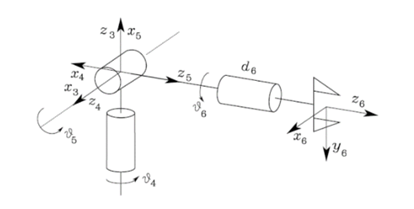
\includegraphics[width=0.6\textwidth]{Image/1.png}
	\caption{球形腕示意图}
\end{figure}
\begin{figure}[h]
	\centering
	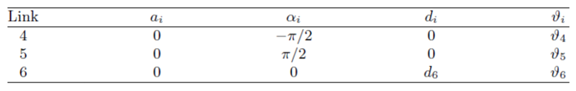
\includegraphics[width=0.8\textwidth]{Image/2.png}
\end{figure}

\subsection{$^6J$的计算}

\textbf{[Solution]:}
由Davis-Hartenberg参数表,可得到各个关节的变换矩阵为:
\begin{equation*}
	^3T_4=\begin{bmatrix}
		cos \theta_4 & -sin \theta_4 & 0 & 0 \\
		0 & 0 & 1 & 0 \\
		-sin \theta_4 & -cos \theta_4 & 0 & 0 \\
		0 & 0 & 0 & 1
	\end{bmatrix} ;
	^4T_5=\begin{bmatrix}
		cos \theta_5 & -sin \theta_5 & 0 & 0 \\
		0 & 0 & -1 & 0 \\
		sin \theta_5 & cos \theta_5 & 0 & 0 \\
		0 & 0 & 0 & 1
	\end{bmatrix} ;
	^5T_6=\begin{bmatrix}
		cos \theta_6 & -sin \theta_6 & 0 & 0 \\
		sin \theta_6 & cos \theta_6 & 0 & 0 \\
		0 & 0 & 1 & d_6\\
		0 & 0 & 0 & 1
	\end{bmatrix}
\end{equation*}

再进行关键变换矩阵的运算:

\begin{equation*}
	^3T_6=^3T_4 \cdot ^4T_5 \cdot ^5T_6 = \begin{bmatrix}
		c_4c_5c_6-c_4s_5s_6 & -c_4c_5s_6-c_4s_5c_6 & s_4 & d_6s_4 \\
		s_5c_6+c_5s_6 & -s_5s_6+c_5c_6 & 0 & 0 \\
		-s_4c_5c_6+s_4s_5s_6 & s_4c_5s_6+s_4s_5c_6 & c_4 & d_6c_4 \\
		0 & 0 & 0 & 1
	\end{bmatrix}
	=\begin{bmatrix}
		c_4c_{56} & -c_4s_{56} & s_4 & d_6s_4 \\
		s_{56} & c_{56} & 0 & 0 \\
		-s_4c_{56} & s_4s_{56} & c_4 & d_6c_4 \\
		0 & 0 & 0 & 1
	\end{bmatrix}
\end{equation*}

为了简化描述,上式中,$s_5 = sin \theta_5 ,s_{56} = sin (\theta_5+\theta_6)$,以此类推。

同样地,
\begin{equation}
	^4T_6=^4T_5 \cdot ^5T_6 = \begin{bmatrix}
		c_{56} & -s_{56} & 0 & 0 \\
		0 & 0 & -1 & -d_6 \\
		s_{56} & c_{56} & 0 & 0 \\
		0 & 0 & 0 & 1
	\end{bmatrix} ;
	^5T_6=\begin{bmatrix}
		c_6 & -s_6 & 0 & 0 \\
		s_6 & c_6 & 0 & 0 \\
		0 & 0 & 1 & d_6\\
		0 & 0 & 0 & 1
	\end{bmatrix}
\end{equation}

由于全部都是旋转关节,因此有:
\begin{equation}
	^TJ(q) = \begin{bmatrix}
		\boldsymbol{^TJ_{li}}\\
		\boldsymbol{^TJ_{ai}}
	\end{bmatrix}
	=\begin{bmatrix}
		(\boldsymbol{p}\times \boldsymbol{n})_z\\
		(\boldsymbol{p}\times \boldsymbol{o})_z\\
		(\boldsymbol{p}\times \boldsymbol{a})_z\\
		\boldsymbol{n}_z\\
		\boldsymbol{o}_z\\
		\boldsymbol{a}_z
	\end{bmatrix}
\end{equation}

对于第三列(对应矩阵$^5T_6$),有:
\begin{equation}
	\begin{aligned}
		&\boldsymbol{n} = \begin{bmatrix}
			c_6 & s_6 & 0
		\end{bmatrix}^T, \boldsymbol{o} = \begin{bmatrix}
			-s_6 & c_6 & 0	
		\end{bmatrix}^T, \boldsymbol{a} = \begin{bmatrix}
			0 & 0 & 1
		\end{bmatrix}^T, \boldsymbol{p} = \begin{bmatrix}
			0 & 0 & d_6
		\end{bmatrix}^T\\
		&\boldsymbol{p}\times \boldsymbol{n} = \left| \begin{matrix}
			i & j & k \\
			0 & 0 & d_6 \\
			c_6 & s_6 & 0
		\end{matrix} \right|_z = 0, \boldsymbol{p}\times \boldsymbol{o} = \left| \begin{matrix}
			i & j & k \\
			0 & 0 & d_6 \\
			-s_6 & c_6 & 0
		\end{matrix} \right|_z = 0, \boldsymbol{p}\times \boldsymbol{a} = \left| \begin{matrix}
			i & j & k \\
			0 & 0 & d_6 \\
			0 & 0 & 1
		\end{matrix} \right|_z = 0\\
	\end{aligned}
\end{equation}

thus,
\begin{equation*}
^6J_{3} = \begin{bmatrix}
	0 & 0 & 0 & 0 & 0 & 1
\end{bmatrix}^T
\end{equation*}

同样的道理,对于第二列(对应矩阵$^4T_6$),有:
\begin{equation*}
	\begin{aligned}
		&\boldsymbol{n} = \begin{bmatrix}
			c_{56} & 0 & s_{56}
		\end{bmatrix}^T, \boldsymbol{o} = \begin{bmatrix}
			-s_{56} & 0 & c_{56}
		\end{bmatrix}^T, \boldsymbol{a} = \begin{bmatrix}
			0 & -1 & 0
		\end{bmatrix}^T, \boldsymbol{p} = \begin{bmatrix}
			0 & -d_6 & 0
		\end{bmatrix}^T\\
	\end{aligned}
\end{equation*}
\begin{equation}
	\begin{aligned}
		&\boldsymbol{p}\times \boldsymbol{n} = \left| \begin{matrix}
			i & j & k \\
			0 & -d_6 & 0 \\
			c_{56} & 0 & s_{56}
		\end{matrix} \right|_z = d_6s_{56},\\& \boldsymbol{p}\times \boldsymbol{o} = \left| \begin{matrix}
			i & j & k \\
			0 & -d_6 & 0 \\
			-s_{56} & 0 & c_{56}
		\end{matrix} \right|_z = -d_6s_{56}, \\&\boldsymbol{p}\times \boldsymbol{a} = \left| \begin{matrix}
			i & j & k \\
			0 & -d_6 & 0 \\
			0 & -1 & 0
		\end{matrix} \right|_z = 0\\
	\end{aligned}
\end{equation}

thus,
\begin{equation*}
^6J_{2} = \begin{bmatrix}
	d_6s_{56} & -d_6s_{56} & 0 & s_{56} & c_{56} & 0
\end{bmatrix}^T
\end{equation*}

最后,对于第一列(对应矩阵$^3T_6$),有:
\begin{equation*}
	\begin{aligned}
		&\boldsymbol{n} = \begin{bmatrix}
			c_4c_{56} & s_{56} & -s_4c_{56}
		\end{bmatrix}^T, \boldsymbol{o} = \begin{bmatrix}
			-c_4s_{56} & c_{56} & s_4s_{56}
		\end{bmatrix}^T, \boldsymbol{a} = \begin{bmatrix}
			s_4 & 0 & c_4
		\end{bmatrix}^T, \boldsymbol{p} = \begin{bmatrix}
			d_6s_4 & 0 & d_6c_4
		\end{bmatrix}^T\\
	\end{aligned}
\end{equation*}
\begin{equation}
	\begin{aligned}
		&\boldsymbol{p}\times \boldsymbol{n} = \left| \begin{matrix}
			i & j & k \\
			d_6s_4 & 0 & d_6c_4 \\
			c_4c_{56} & s_{56} & -s_4c_{56}
		\end{matrix} \right|_z = d_6c_4s_{56},\\& \boldsymbol{p}\times \boldsymbol{o} = \left| \begin{matrix}
			i & j & k \\
			d_6s_4 & 0 & d_6c_4 \\
			-c_4s_{56} & c_{56} & s_4s_{56}
		\end{matrix} \right|_z = d_6s_4c_{56}, \\&\boldsymbol{p}\times \boldsymbol{a} = \left| \begin{matrix}
			i & j & k \\
			d_6s_4 & 0 & d_6c_4 \\
			s_4 & 0 & c_4
		\end{matrix} \right|_z = 0\\
	\end{aligned}
\end{equation}
thus,
\begin{equation*}
^6J_{1} = \begin{bmatrix}
	d_6c_4s_{56} & d_6s_4c_{56} & 0 & -s_4c_{56} & s_4s_{56} & c_4
\end{bmatrix}^T
\end{equation*}

综上所述,$^6J$为:
\begin{equation}
	^6J (q)= \begin{bmatrix}
		^6J_1 & ^6J_2 & ^6J_3
	\end{bmatrix} = \begin{bmatrix}
		d_6c_4s_{56} & d_6s_{56} & 0\\
		d_6s_4c_{56} & -d_6s_{56} & 0\\
		0 & 0 & 0 \\
		-s_4c_{56} & s_{56} & 0\\
		s_4s_{56} & c_{56} & 0\\
		c_4 & 0 & 1
	\end{bmatrix}
\end{equation}

\subsection{$^3J$的计算}

\textbf{[Solution]:}
对于$^3J$的计算,由关系式
\begin{equation}
	^3J (q)= \begin{bmatrix}
		^3R_6 & 0\\
		0 & ^3R_6
	\end{bmatrix} \cdot ^6J(q)
\end{equation}

因为旋转矩阵为\textbf{正交矩阵},有$^3R_6 = (^6R_3)^{-1} = ^3R_6^T$,因此有:
\begin{equation*}
	^3R_6 = \begin{bmatrix}
		c_4c_{56} & s_{56} & -s_4c_{56}\\
		-c_4s_{56} & c_{56} & s_4s_{56}\\
		s_4 & 0 & c_4
	\end{bmatrix}
\end{equation*}

因此,$^3J$为:
\begin{equation}
	\begin{aligned}
	^3J (q)&= \begin{bmatrix}
		^3R_6 & 0\\
		0 & ^3R_6
	\end{bmatrix} \cdot ^6J(q) \\
	&= \begin{bmatrix}
		c_4c_{56} & s_{56} & -s_4c_{56} & 0 & 0 & 0\\
		-c_4s_{56} & c_{56} & s_4s_{56} & 0 & 0 & 0\\
		s_4 & 0 & c_4 & 0 & 0 & 0\\
		0 & 0 & 0 & c_4c_{56} & s_{56} & -s_4c_{56}\\
		0 & 0 & 0 & -c_4s_{56} & c_{56} & s_4s_{56}\\
		0 & 0 & 0 & s_4 & 0 & c_4
	\end{bmatrix}
	\begin{bmatrix}
		d_6c_4s_{56} & d_6s_{56} & 0\\
		d_6s_4c_{56} & -d_6s_{56} & 0\\
		0 & 0 & 0 \\
		-s_4c_{56} & s_{56} & 0\\
		s_4s_{56} & c_{56} & 0\\
		c_4 & 0 & 1
	\end{bmatrix}\\
	&= \begin{bmatrix}
		^3J_{11} & ^3J_{12} & ^3J_{13}\\
		^3J_{21} & ^3J_{22} & ^3J_{23}\\
		^3J_{31} & ^3J_{32} & ^3J_{33}\\
		^3J_{41} & ^3J_{42} & ^3J_{43}\\
		^3J_{51} & ^3J_{52} & ^3J_{53}\\
		^3J_{61} & ^3J_{62} & ^3J_{63}
	\end{bmatrix}
\end{aligned}
\end{equation}

其中,各个元素的值为:
\begin{equation}
	\begin{aligned}
		&^3J_{11} = c_4c_{56}d_6c_4s_{56} +s_{56}d_6s_4c_{56} = d_6s_{56}(c_4^2+c_{56}s_4)\\
		&^3J_{12} = c_4c_{56}d_6s_{56} -s_{56}d_6s_4c_{56} = d_6s_{56}(c_4c_{56}-s_{56})\\
		&^3J_{21} = -c_4s_{56}d_6c_4s_{56} -c_{56}d_6s_4s_{56} = -d_6s_{56}(c_4^2s_{56}+c_{56})\\
		&^3J_{22} = -c_4s_{56}d_6s_{56} - c_{56}d_6s_4s_{56} = -d_6s_{56}(c_4s_{56}+c_{56})\\
		&^3J_{31} = s_4d_6c_4s_{56} \\
		&^3J_{32} = s_4d_6s_{56} \\
		&^3J_{41} = -c_4c_{56}s_4c_{56} + s_{56}s_4s_{56} = -s_4(c_56c_4^2+s_{56}^2)\\
		&^3J_{42} = -c_4c_{56}s_{56}+s_{56}c_{56}\\
		&^3J_{51} = c_4s_{56}s_4c_{56} + c_{56}s_4s_{56}+s_4s_{56}c_4\\
		&^3J_{52} = -c_4s_{56}s_{56}+c_{56}^2\\
		&^3J_{61} = -s_4^2c_{56} + c_4^2\\
		&^3J_{62} = s_4s_{56}\\
		&^3J_{13} = 0,^3J_{23} = 0,^3J_{33} = 0\\
		&^3J_{43} = -s_4c_{56} ,^3J_{53} = s_4s_{56},^3J_{63} = c_4\\
	\end{aligned}
\end{equation}

以上,求解完毕。
\end{document}

